\subsection{Experimental overview of Bottomonia results at RHIC and LHC}

The primary motivation for studying high-energy heavy ion collisions is to better understand the hot and dense
matter produced in these interactions. Lattice quantum chromodynamics (LQCD) calculations indicate that at
sufficiently high temperatures a crossover occurs from hadronic matter to a strongly interacting system
of deconfined quarks and gluons known as ``quark-gluon plasma'' (QGP). One of the most prominent signatures of QGP
formation is that the production of quarkonia, the bound states of a heavy quark and its antiquark, is suppressed
with respect to expectations from scaling the yields in proton-proton collisions by the number of binary nucleon-nucleon
(NN) collisions. This suppression arises because the quarkonia binding is weakened by color screening caused by
the surrounding partons in the medium~\cite{Matsui:1986dk}. Therefore the extent of the quarkonia suppression is
expected to be sequentially ordered by the binding energies of the quarkonia states. Because of the binding energy
dependence of the screening, the bottomonium states ($\Upsilon$(1S), $\Upsilon$(2S),
$\Upsilon$(3S), $\chi_{b}$, etc.) are particularly useful probes to understand the space-time evolution
of the QGP. The sequential suppression of the yield of $\Upsilon$(nS) states was first observed by
CMS at $\sNN =$2.76 TeV~\cite{Chatrchyan:2011pe,Chatrchyan:2012lxa}. More recently, results with improved
statistical precision have been reported by both the ALICE and CMS Collaborations at $\sNN =$5.02
TeV~\cite{ALICE:2018wzm,Sirunyan:2018nsz,Sirunyan:2017lzi}. The suppression of the $\Upsilon$(1S)
meson has also been studied at $\sNN =$200 GeV at RHIC~\cite{STAR:2013kwk}.

The screening due to the QGP can also result in an azimuthal asymmetry in the observed yields of quarkonia. In non-central
heavy ion collisions, the produced QGP has a lenticular shape in the transverse plane. Consequently, the average path length
for quarkonia traveling through the medium depends on the direction taken with respect to this shape, with a larger suppression
in the direction of the longer axis~\cite{He:2015hfa}. The anisotropic distribution of particles can be characterized by the magnitudes
of the Fourier co-efficients (v$_{n}$) of the azimuthal correlation of particles~\cite{Voloshin:1994mz}. By studying the
azimuthal distribution of the quarkonia, it is possible to develop a more comprehensive understanding of the dynamics of their
production. The available experimental data, spanning from 0.20 to 5.02 TeV, have provided new insight into the thermal properties
of the QGP. In this section we review the current status of the experimental measurement of R$_{AA}$ and v$_{2}$ for
$\Upsilon$ states. The data from different experiments are comapred and physics insights from them is discussed.   



%\subsubsection{Proton-proton collisions as a reference for R$_{AA}$ at the LHC}




\subsubsection{$\Upsilon$(nS) R$_{AA}$ at the LHC}


\paragraph{Measurement by CMS, ATLAS and ALICE}

The bottomonia states ($\Upsilon$(nS)) are measured at the LHC with very good statistical
precision~\cite{Chatrchyan:2012lxa,Abelev:2014nua,Chatrchyan:2011pe,Khachatryan:2016xxp}.
The CMS measurements at $\sNN =$2.76 TeV~\cite{Chatrchyan:2012lxa,Chatrchyan:2011pe} reveal
a clear proof of sequential suppression :  $\Upsilon$(2S) and $\Upsilon$(3S) are 
more suppressed relative to the ground state $\Upsilon$(1S).   The individual $\Upsilon$ states are also found to be suppressed in
the PbPb collisions relative to the production in the pp collisions. The $\Upsilon$ nuclear
modification factor, $R_{AA}$, shows a strong dependence on collision centrality but has
weak dependence on $\Upsilon$ meson $\pT$ and rapidity~\cite{Khachatryan:2016xxp}.
The forward rapidity ($2.5 \leq y^{\Upsilon} \leq 4.0$) measurement of the $\Upsilon$ suppression at 
ALICE~\cite{Abelev:2014nua} is found to be consistent with the midrapidity ($|y^{\Upsilon}|\,\leq 2.4$)
measurement of the $\Upsilon$ suppression at the CMS. 
The CMS and ALICE collaborations have carried out the $R_{AA}$ measurement of $\Upsilon$
at $\sNN =$ 5.02 TeV with the Run II LHC PbPb
collisions~\cite{Sirunyan:2018nsz,Sirunyan:2017lzi,ALICE:2018wzm}.
The CMS experiment measured slightly more amount of $\Upsilon$ suppression at
$\sNN =$ 5.02 TeV~\cite{Sirunyan:2018nsz,Sirunyan:2017lzi} than the suppression at
$\sNN =$ 2.76 TeV~\cite{Khachatryan:2016xxp} while the ALICE experiment observed less
suppression at $\sNN =$ 5.02 TeV than that at $\sNN =$ 2.76 TeV 
in the most central PbPb collisions~\cite{Abelev:2014nua,ALICE:2018wzm}. 

\subsubsection{$\Upsilon$(nS) azimuthal anisotropy at the LHC}

\begin{figure}
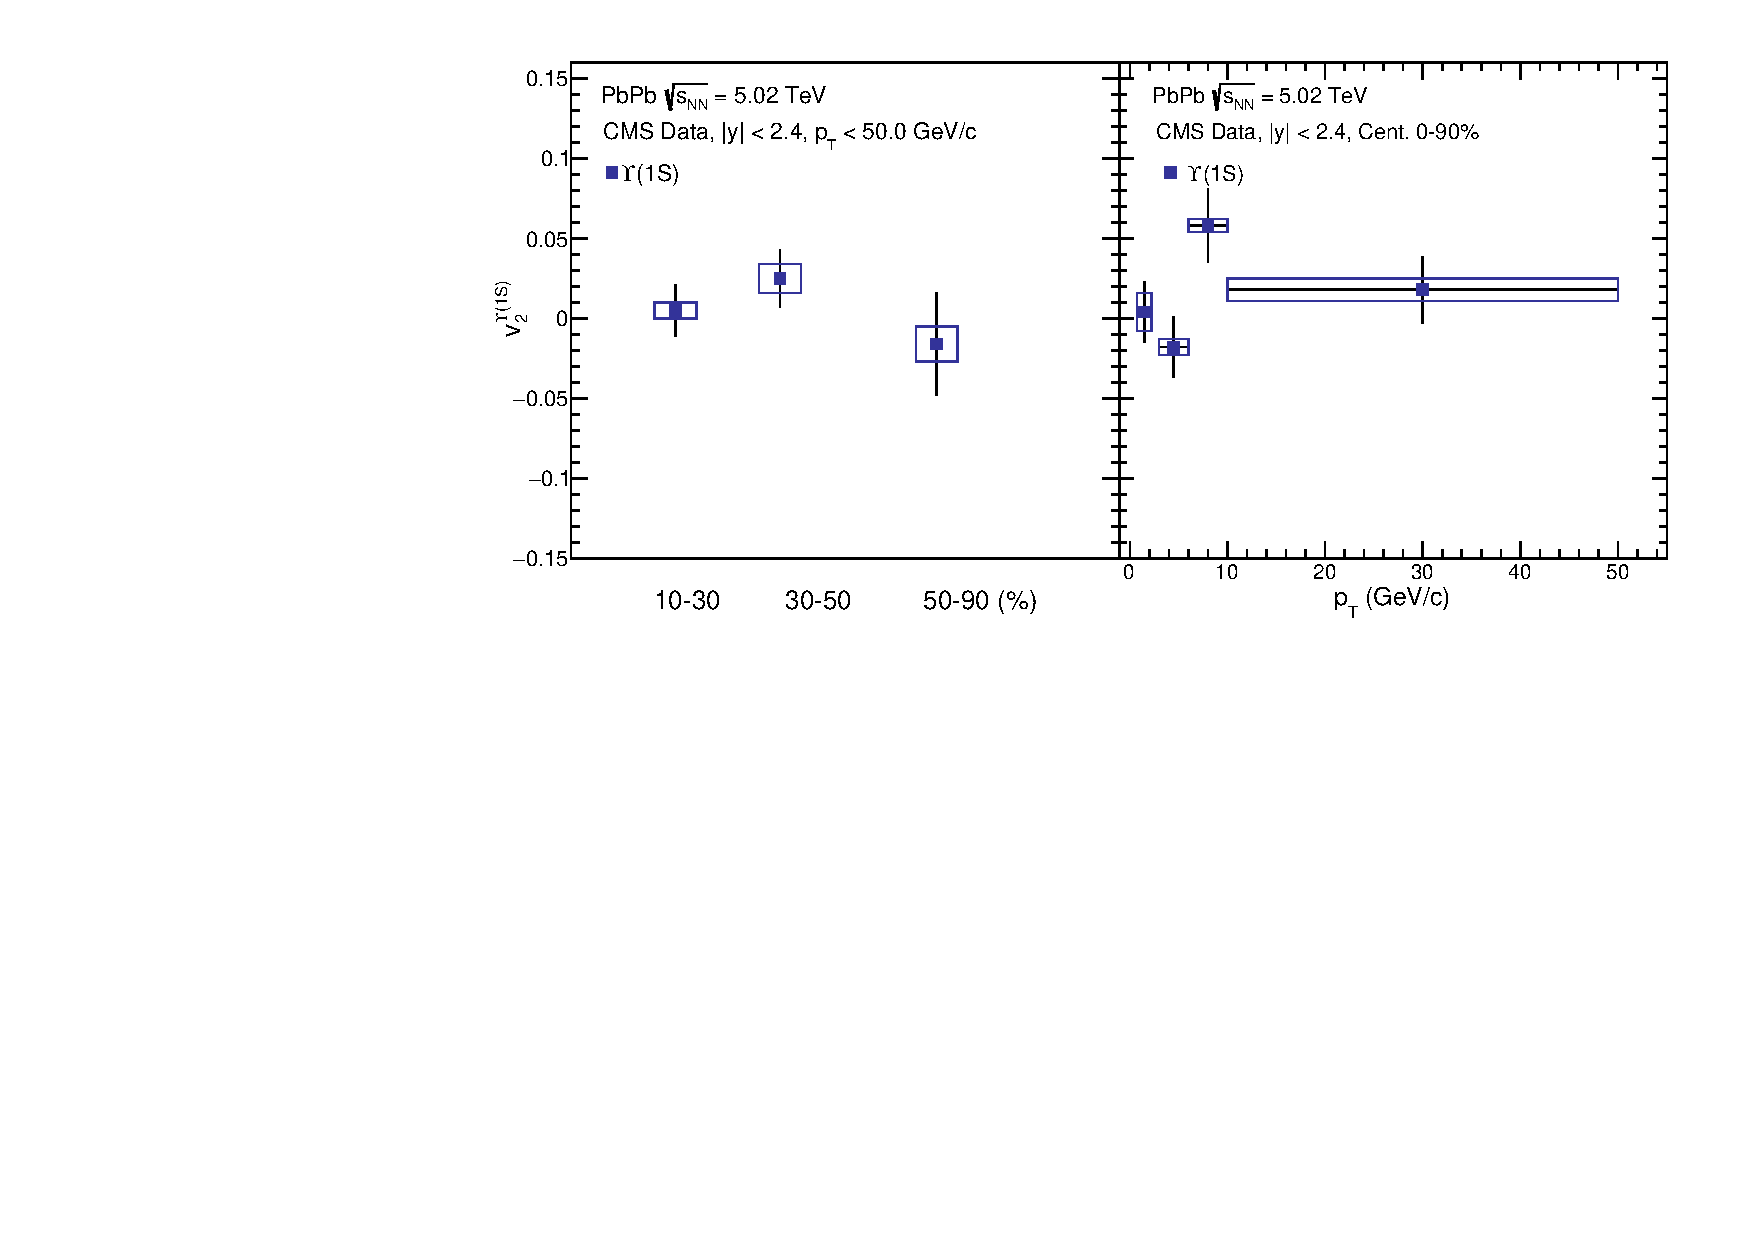
\includegraphics[width=0.99\textwidth]{Figures/ExpOverview/Fig_CMS_Y1S_5TeV_V2.pdf}
\caption{(Color online) The $\Upsilon$(1S) azimuthal anisotropy (v$_{2}$) (a) as a function of collision centrality and 
  (b) as a function of transverse momentum $p_{T}$~\cite{CMS:2020efs}.
}
\label{fig:Upsilon1SV2CMS}
\end{figure}


Figure~\ref{fig:Upsilon1SV2CMS} shows the $\Upsilon$(1S) azimuthal anisotropy (v$_{2}$) (a) as a function of collision centrality and 
(b) as a function of transverse momentum $p_{T}$ measured by CMS experiment at LHC~\cite{CMS:2020efs}. The p$_{T}$ integrated results
shown in Fig.~\ref{fig:Upsilon1SV2CMS} (a) for three centrality intervals are consistent with zero within the statistical
uncertainties. The p$_{T}$ dependence of $\Upsilon$(1S) meson v$_{2}$ values is measured for the 10-90$\%$ centrality interval.
The v$_{2}$ values are consistent with zero in the measured p$_T$ range, except for the 6$<$p$_{T}<$10 GeV/c interval that
shows a 2.6$\sigma$ deviation from zero. 







\paragraph{Measurement by CMS and ATLAS}

\subsubsection{$\Upsilon$(nS) R$_{AA}$ at the RHIC}

\paragraph{Measurement by STAR and PHENIX}
